\documentclass[a4paper]{article}
\usepackage[utf8x]{inputenc}
\usepackage[T2A]{fontenc}
\usepackage{amsmath}
\usepackage{hyperref}
\usepackage[russian, english]{babel}
\usepackage{graphicx}
\graphicspath{}
\usepackage{float}
\usepackage{tabto}
\usepackage{amsfonts}
\usepackage{amssymb}
\usepackage{bm}
\DeclareGraphicsExtensions{.pdf,.png,.jpg}
\usepackage{biblatex}
\addbibresource{ref.bib}
\hypersetup{unicode=true}
\urlstyle{same}

\begin{document}
\selectlanguage{russian}

\begin{titlepage}
	\clearpage\thispagestyle{empty}
	\centering
	\vspace{1cm}

	% Titles
	% Information about the University
	{\largeСанкт-Петербургский политехнический университет Петра Великого\\
        Институт прикладной математики и механики\\
        Кафедра «Прикладная математика»
    \par}
    
	\vspace{4cm}
	{\huge \textbf{Отчёт по курсовой работе по дисциплине «Вычислительные комплексы»}} \\

	\vspace{4cm}
	{\hfill{} Выполнил студент:\\
	\hfill{}Карасев Александр Андреевич\\
	\hfill{}группа: 3630102/70201}\vspace{2cm}
	
    {\hfill{} Проверил:\\
	\hfill{}к.ф.-м.н.,доцент\\
	\hfill{}Баженов Александр Николаевич}
	
	
	\vspace{2cm}
    \centering{Санкт-Петербург}

	{\normalsize 2020г. \par}
	
	\pagebreak

\end{titlepage}

\tableofcontents
\pagebreak

\section{Постановка задачи}
Для демонстрации интервальной глобальной минимизации использовать функцию:
\begin{equation}
function[Z;WorkList] = globopt0(X)    
\end{equation}
Она возвращает значение глобального экстремумуа Z и рабочий список WorkList. Работа алгоритма построена на последовательном сужении множества, на котором строится оптимум.
\section{Теория}
Алгоритм для глобальной минимизации функции GlobOpt оперирует с рабочим списком $\zeta$, в котором будут храниться брусы, получающиеся в результате дробления исходного бруса области определения на более мелкие подбрусы.\\
Одновременно с самими подбрусами будем хранить в рабочем списке и нижние оценки областей значений целевой функции по этим подбрусам, так что элементам списка $\zeta$ будут записи-пары вида:
\begin{equation}
    \zeta: (Y, y), \text{ где } Y \subseteq X, \; y = f(Y)
\end{equation}
Далее каждый шаг алгоритма состоит в извлечении из этого списка брус, который обеспечивает рекордную (т.е. наименьшую) на данный момент оценку минимума снизу, его дроблении на более мелкие подбрусы, оценивании на них целевой функции, занесении результатов обратно в рабочий список.
\section{Результаты}
Были рассмотрены следующие функции:
\begin{itemize}
    \item Функция Бута
    \begin{equation*}
        f(x, y) = (x + 2y − 7)^2 + (2x + y − 5)^2
    \end{equation*}
    Имеет минимум 0 в $X = (1, 3)$
    \item Функция CrossInTray
    \begin{equation*}
        f(x, y) = -0.0001[|sin(x)sin(y)exp(|100 - \frac{\sqrt{x^2+y^2}}{\pi}|)|+1]^{0.1}
    \end{equation*}
    Имеет минимум 2.0626 в $X = (\pm 1.3494, \pm 1.3494)$
    \item Функция Химмельблау
    \begin{equation*}
        f(x, y) = (x^2 + y - 11)^2 + (x + y^2 - 7)^2
    \end{equation*}
    Имеет минимум 0 в $X = (3, 2)$
    \item Функция Хёльдера
    \begin{equation*}
        f(x, y) = -1 \cdot |sin(x)cos(y) exp(|1 -\frac{\sqrt{x^2+y^2}}{\pi}|)|
    \end{equation*}
    Имеет минимум -19.2085 в  $X = (\pm 8.05502, \pm 9.66459)$
    \item Функция Растригина
    \begin{equation*}
        f(x, y) = x^2 + y^2 - cos(18x) - cos(18y)
    \end{equation*}
    Имеет минимум -2 в $X = (0, 0)$
    \item Функция Розенброка
    \begin{equation*}
        f(x, y) = 100 (x^2 - y)^2 - (x - 1)^2
    \end{equation*}
    Имеет минимум 0 в $X = (1, 1)$
    \item Параболоид
    \begin{equation*}
        f(x, y) = x^2 + y^2
    \end{equation*}
    Имеет минимум 0 в $X = (0, 0)$
\end{itemize}
Следуя описанному алгоритму были получены следующие результаты. \\
\newpage
Рассмотрим положения брусов из рабочего списка алгоритма и положения их центров для различных входных функций. 
\begin{figure}[H]
\begin{minipage}[h]{0.5\linewidth}
\center{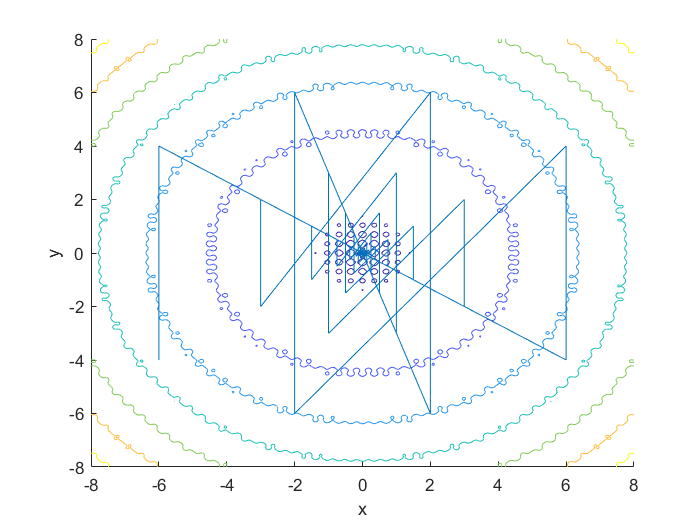
\includegraphics[width=1\linewidth]{Rastr_1.png}} a) \\
\end{minipage}
\hfill
\begin{minipage}[h]{0.5\linewidth}
\center{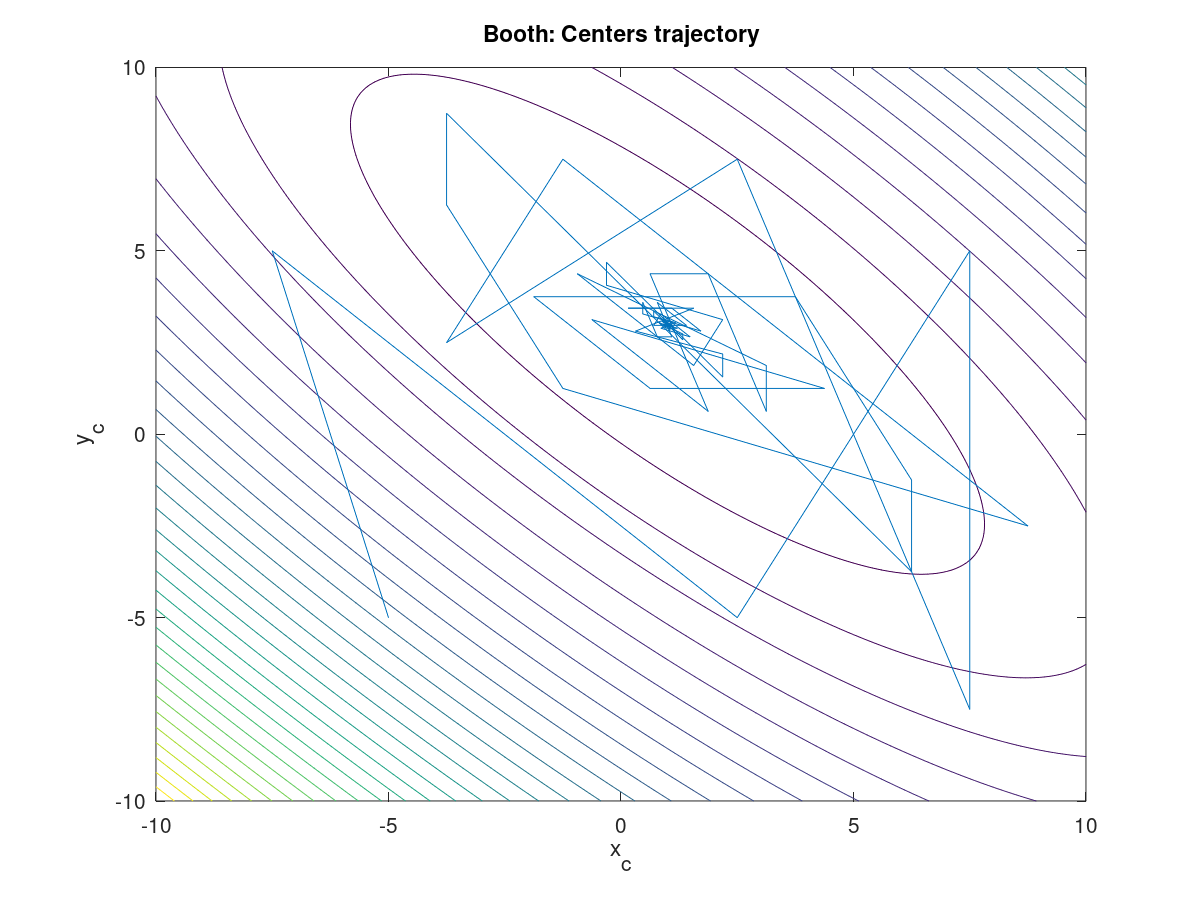
\includegraphics[width=1\linewidth]{Buth_2.png}} \\b)
\end{minipage}
\vfill
\begin{minipage}[h]{0.5\linewidth}
\center{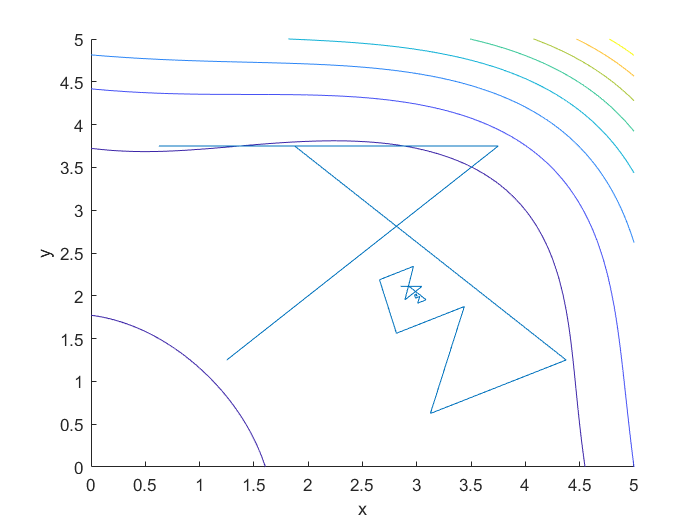
\includegraphics[width=1\linewidth]{Himmelblau_1.png}} c) \\
\end{minipage}
\hfill
\begin{minipage}[h]{0.5\linewidth}
\center{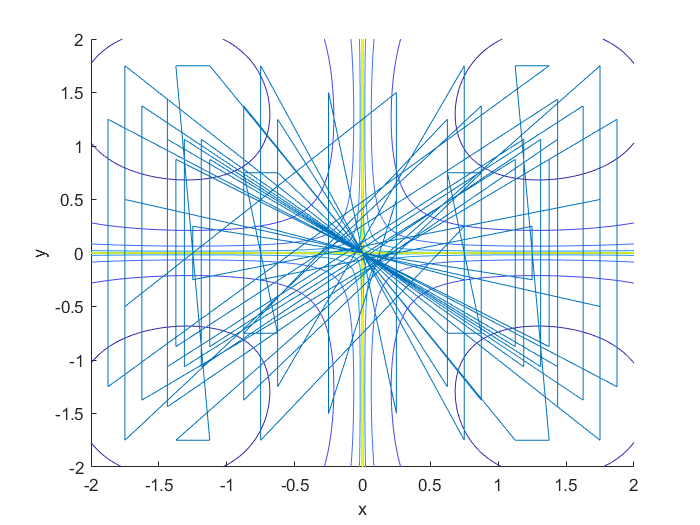
\includegraphics[width=1\linewidth]{crossInTray_1.png}} d) \\
\end{minipage}
\vfill
\begin{minipage}[h]{0.5\linewidth}
\center{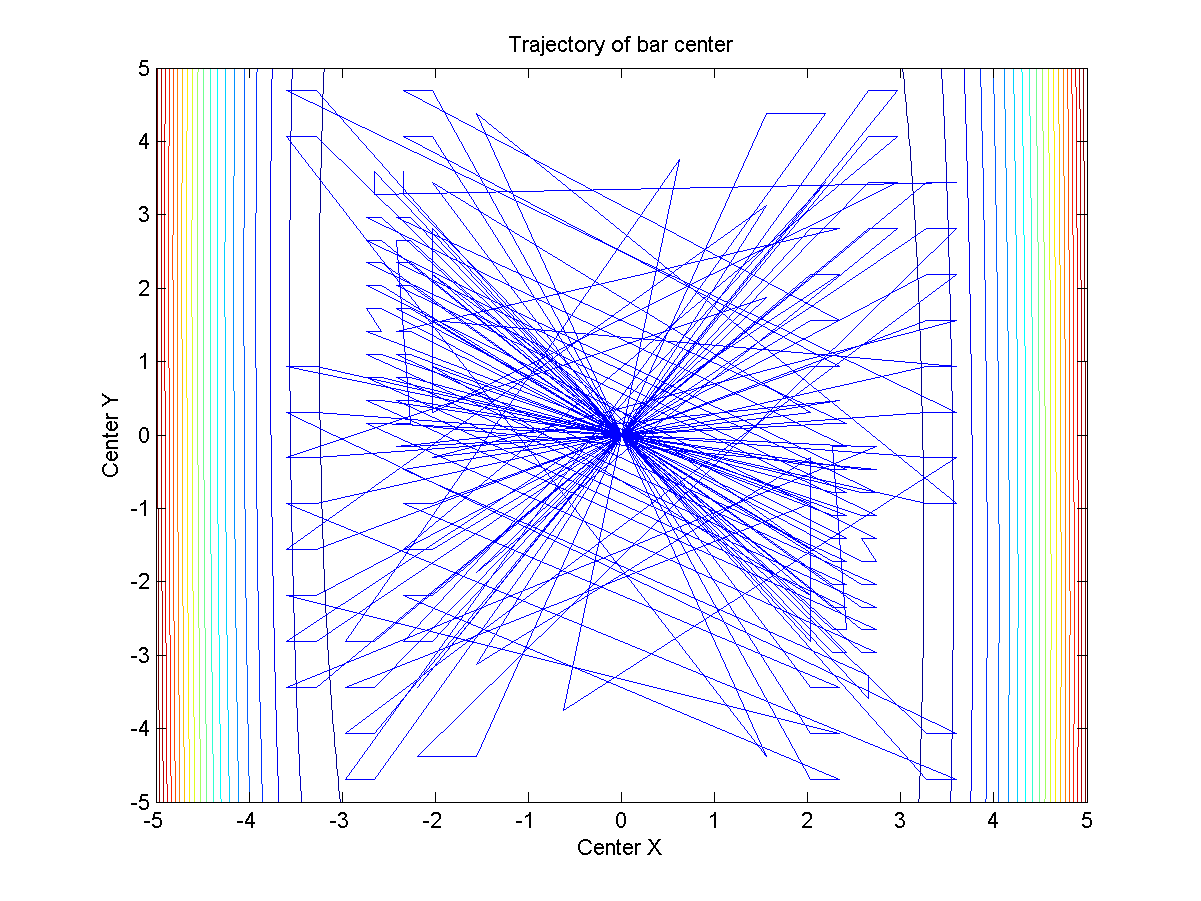
\includegraphics[width=1\linewidth]{ThreeHumpCamel.png}} e) \\
\end{minipage}
\hfill
\begin{minipage}[h]{0.5\linewidth}
\center{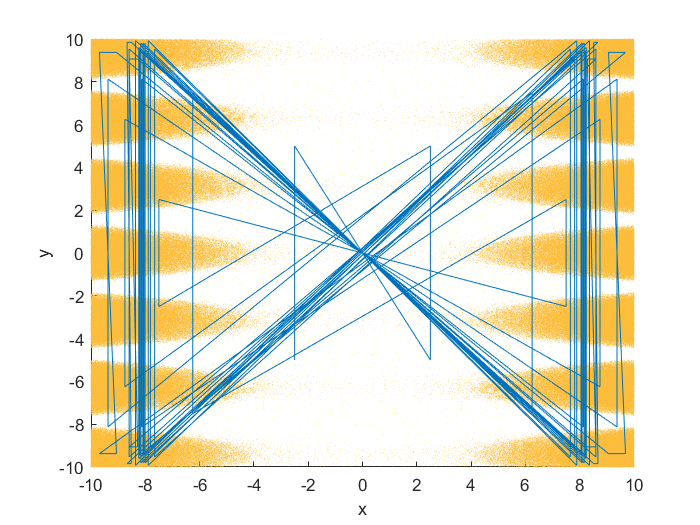
\includegraphics[width=1\linewidth]{Holder_1.png}} \\f)
\end{minipage}
\caption{Положения центров брусов в процессе алгоритма: a) функция Растригина, b)функция Бута, c) функция Химмельблау, d) функция 'cross in tray' , e) функция 'three hump camel' , f)  функция Хёльдера.}
\label{ris:center_blocks}
\end{figure}
\newpage
А теперь рассмотрим графики радиусов рабочих брусов в логарифмическом масштабе.
\begin{figure}[H]
\begin{minipage}[h]{0.5\linewidth}
\center{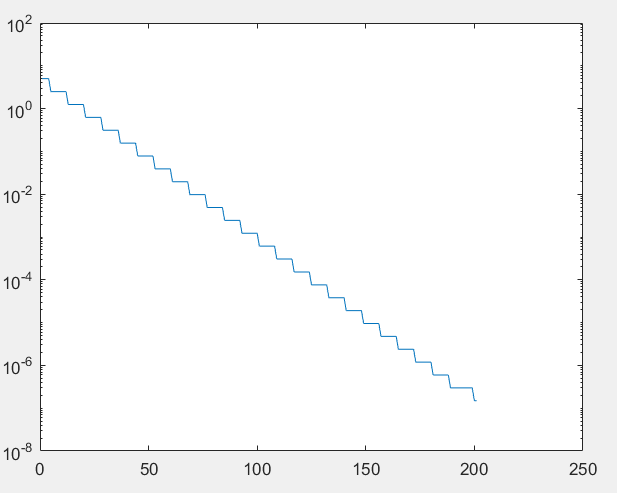
\includegraphics[width=1\linewidth]{Rastr_inter_2.png}} a) \\
\end{minipage}
\hfill
\begin{minipage}[h]{0.5\linewidth}
\center{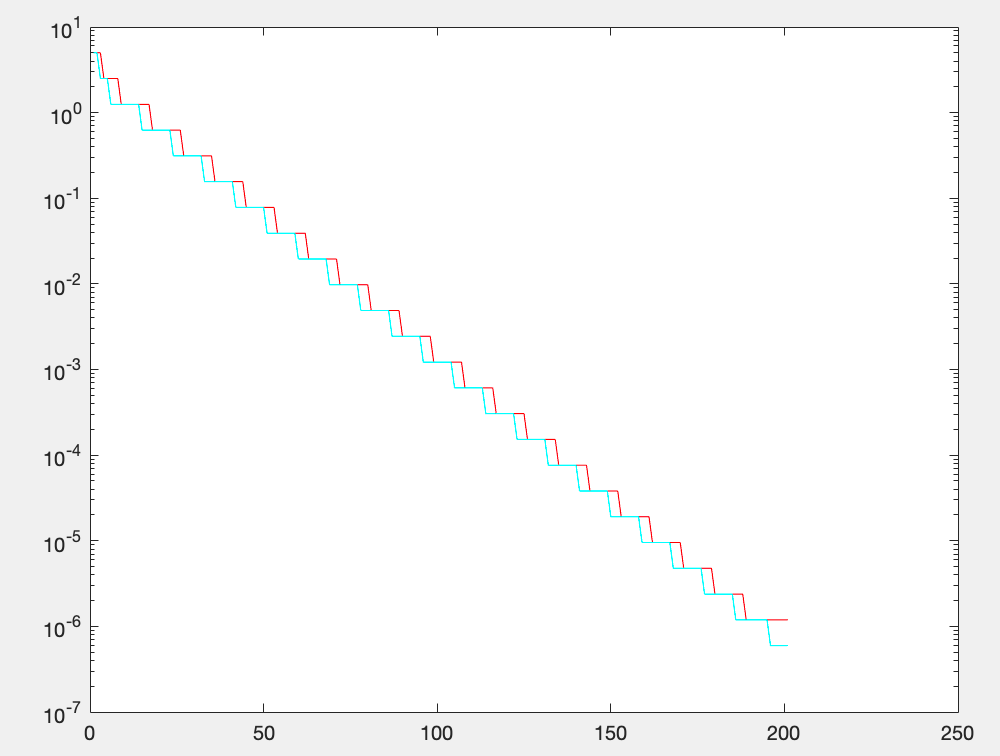
\includegraphics[width=1\linewidth]{Buth_inter_1.png}} \\b)
\end{minipage}
\vfill
\begin{minipage}[h]{0.5\linewidth}
\center{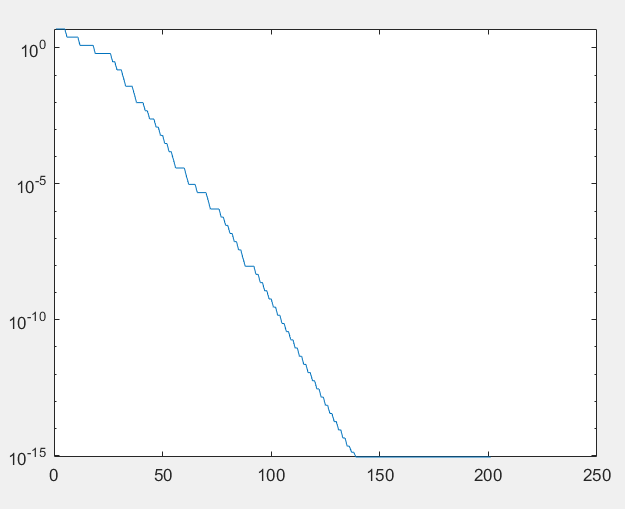
\includegraphics[width=1\linewidth]{Himmelblau_inter_1.png}} c) \\
\end{minipage}
\hfill
\begin{minipage}[h]{0.5\linewidth}
\center{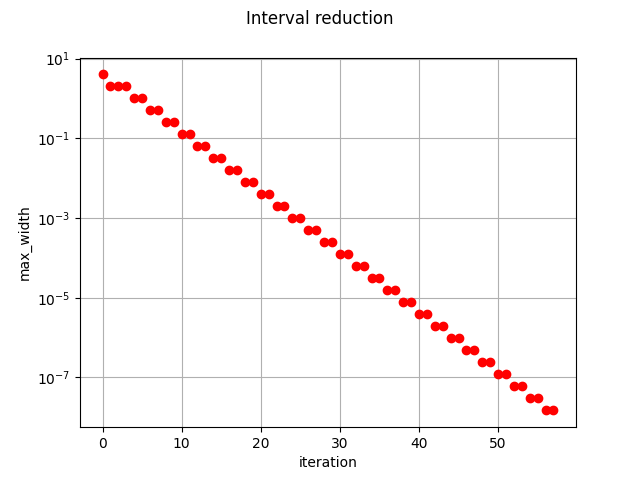
\includegraphics[width=1\linewidth]{Rosen_inter_1.png}} d) \\
\end{minipage}
\vfill
\begin{minipage}[h]{0.5\linewidth}
\center{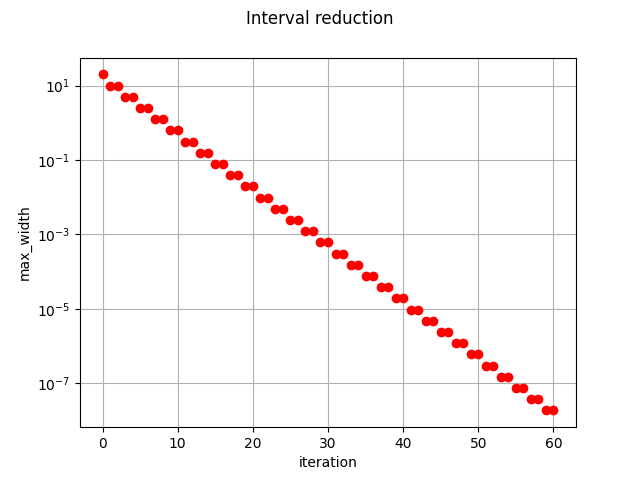
\includegraphics[width=1\linewidth]{Sphere_inter_1.png}} e) \\
\end{minipage}
\caption{Радиусы рабочих брусов в логарифмическом масштабе для: a) функции Растригина, b) функции Бута, c) функции Химмельблау, d) функции Розенброка , e) функции параболоида.}
\label{ris:radius_blocks}
\end{figure}

\newpage
Также рассмотрим сходимость алгоритма для разных функций (измерения расстояния до точки минимума в логарифмических координатах):
\begin{figure}[H]
\begin{minipage}[h]{0.5\linewidth}
\center{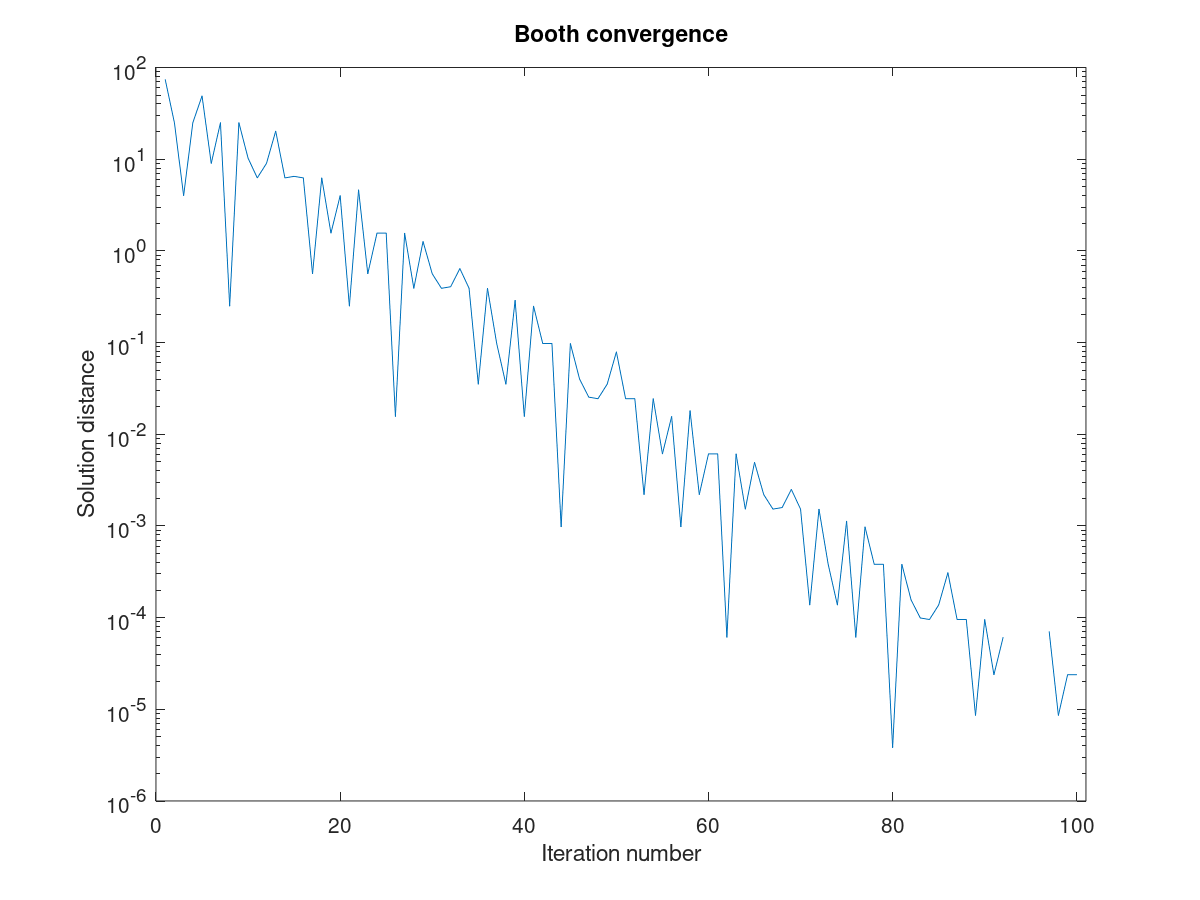
\includegraphics[width=1\linewidth]{Buth_conv_1.png}} a) \\
\end{minipage}
\hfill
\begin{minipage}[h]{0.5\linewidth}
\center{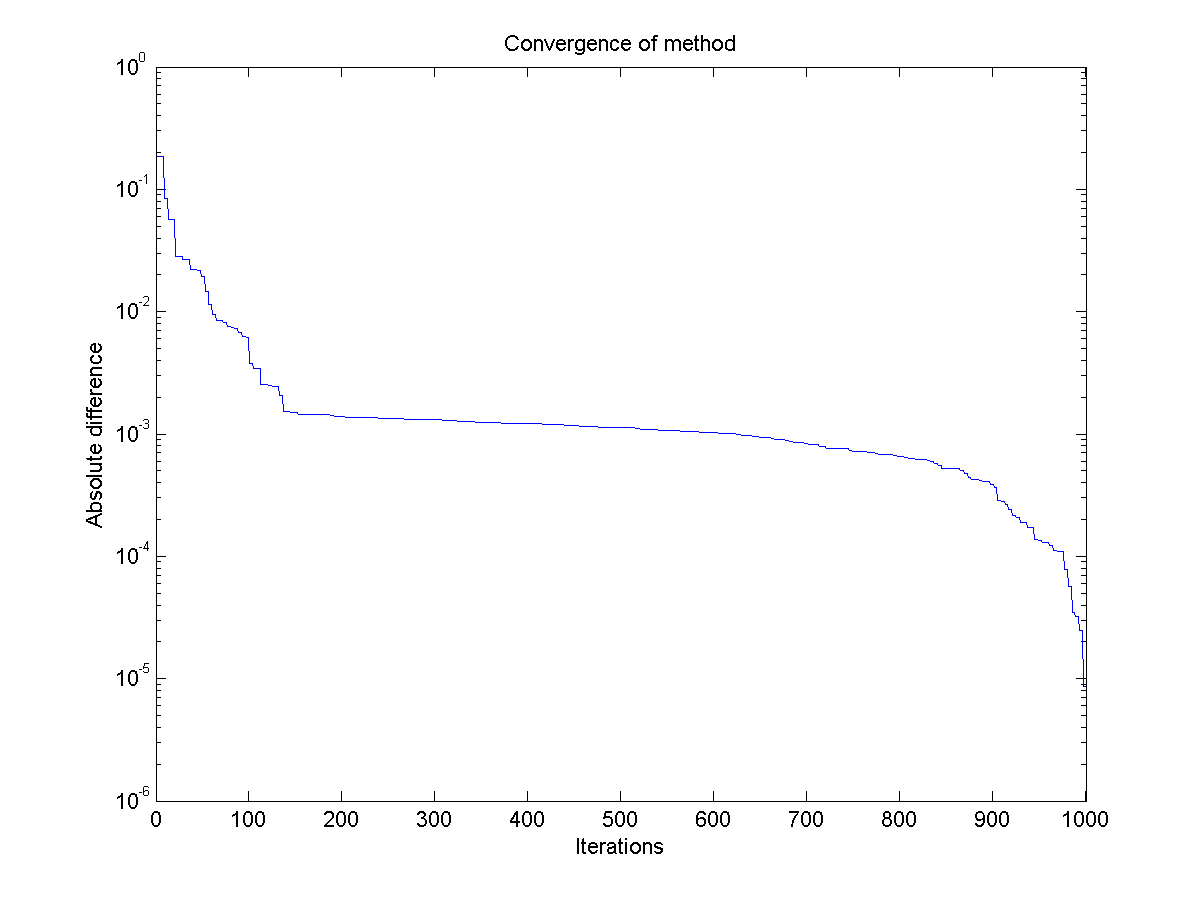
\includegraphics[width=1\linewidth]{CrossInTray_conv_1.png}} \\b)
\end{minipage}
\vfill
\begin{minipage}[h]{0.5\linewidth}
\center{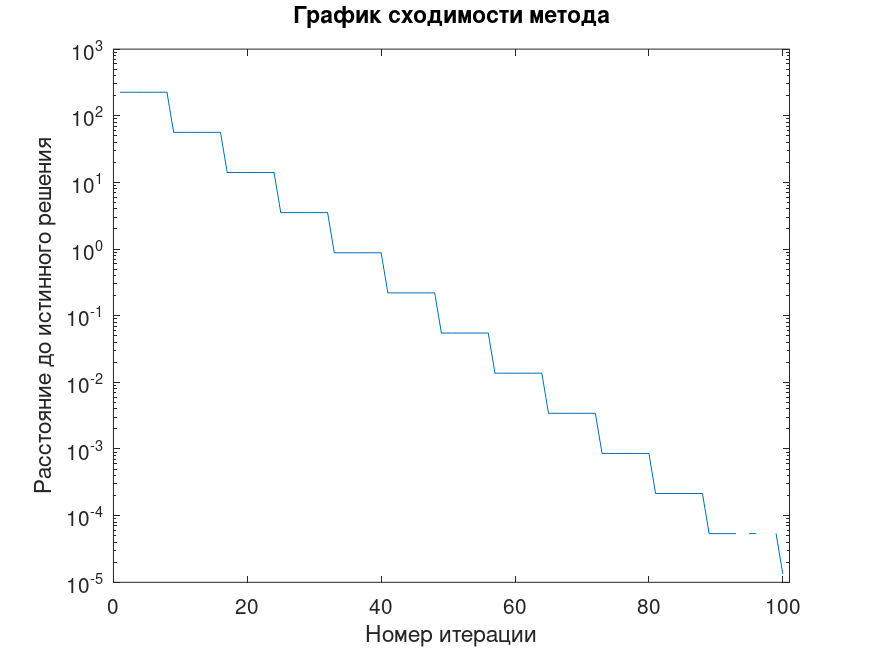
\includegraphics[width=1\linewidth]{sphere_conv_1.png}} c) \\
\end{minipage}
\hfill
\begin{minipage}[h]{0.5\linewidth}
\center{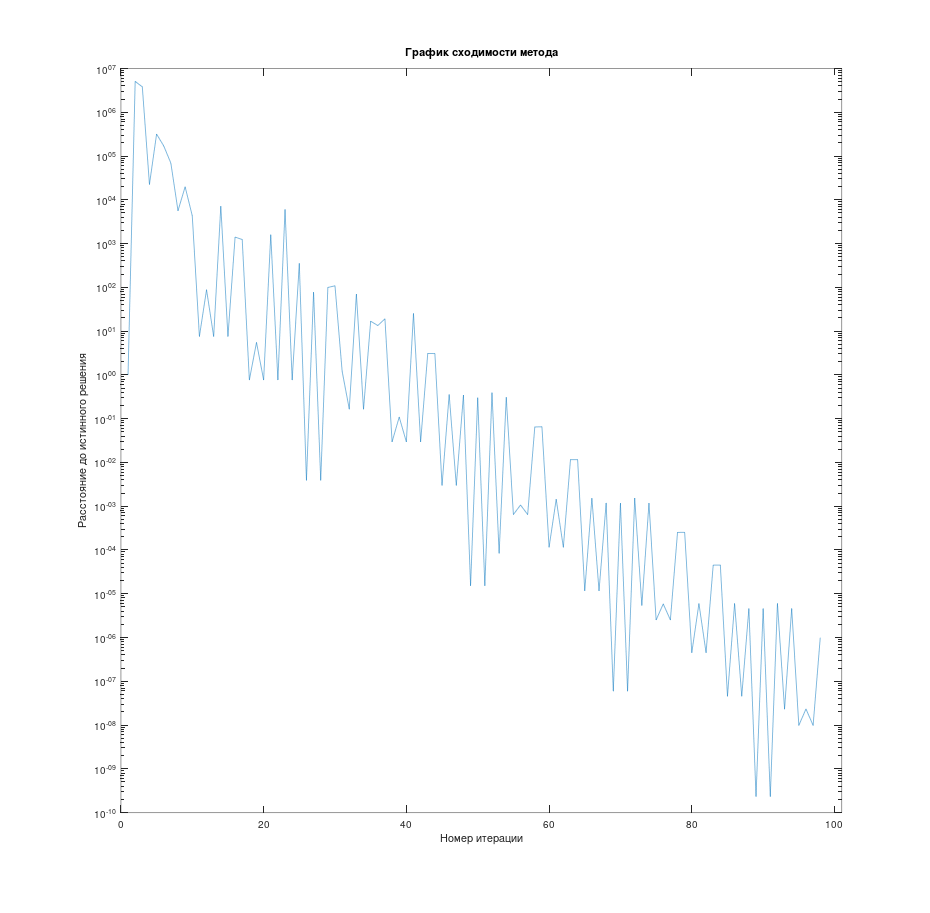
\includegraphics[width=1\linewidth]{Rosen_conv_1.png}} d) 
\end{minipage}
\caption{Расстояние от центра бруса до точки минимума в логарифмическом масштабе: a) функция Бута, b) функция 'cross in tray' , c) функция параболоида, d) функция Розенброка.}
\label{ris:conv_centres_blocks}
\end{figure}

\section{Вывод}
По полученным выводам можно сделать вывод:\\
Радиусы брусов для заданного алгоритма globopt0 уменьшаются линейно в логарифмическом масштабе для всех рассмотренных функций, следовательно логарифмически в линейном масштабе. Это и не удивительно - алгоритм на каждой итерации делит максимальную составляющую пополам.\\
Однако про скорость сходимости данного алгоритму к глобального минимума ничего сказать нельзя - для разных функций он показывал разный результат. Преобладающим результатом является логарифмическая, что является неплохим результатом для такого очевидного и простого в реализации алгоритма. 
\section{Ссылка на github}
Ссылка на гитхаб с документом и входящим в него рисунками:\\
\url{https://github.com/MethaHardworker/Calculation_Complex/tree/main/course}
\end{document}